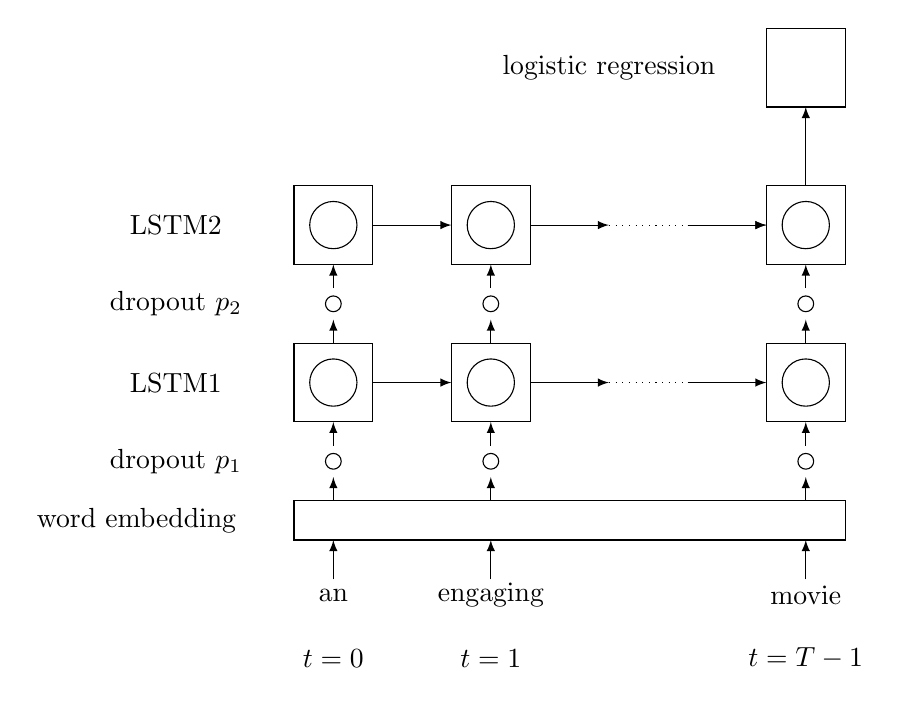
\begin{tikzpicture}
\foreach \x in  {7, 9, 13}
{
	\draw (\x,1) rectangle (\x+1,2);
	\draw (\x,3) rectangle (\x+1,4);
	\draw (\x+0.5,1.5) circle (0.3cm);
	\draw (\x+0.5,3.5) circle (0.3cm);
	\draw [-latex](\x+0.5,0) -- (\x+0.5,0.3);
	\draw [-latex](\x+0.5,0.7) -- (\x+0.5,1.0);
	\draw [-latex](\x+0.5,2) -- (\x+0.5,2.3);
	\draw [-latex](\x+0.5,2.7) -- (\x+0.5,3);
	\draw (\x+0.5,2.5) circle (0.1cm);
	\draw (\x+0.5,0.5) circle (0.1cm);
	\draw [-latex](\x+0.5,-1) -- (\x+0.5,-0.5);
}

\foreach \x in  {9, 11, 13}
{
	\draw [-latex](\x-1,1.5) -- (\x,1.5);
	\draw [-latex](\x-1,3.5) -- (\x,3.5);
}

\draw [-latex](12,3.5) -- (13,3.5);

\path (7.5,-2) node[draw=none] (t0) {$t=0$};
\path (9.5,-2) node[draw=none] (t1) {$t=1$};
\path (13.5,-2) node[draw=none] (tT1) {$t=T-1$};
\draw [dotted] (11,1.5) -- (12,1.5);
\draw [dotted] (11,3.5) -- (12,3.5);

\path (7.5,-1.2) node[draw=none] (w1) {an};
\path (9.5,-1.2) node[draw=none] (w2) {engaging};
\path (13.5,-1.2) node[draw=none] (w3) {movie};
\path (5.5,2.5) node[draw=none] (drop) {dropout $p_2$};
\path (5.5,0.5) node[draw=none] (drop) {dropout $p_1$};
\path (5.5,1.5) node[draw=none] (lstm1) {LSTM1};
\path (5.5,3.5) node[draw=none] (lstm2) {LSTM2};
\path (5,-0.25) node[draw=none] (lstm2) {word embedding};

\draw (13,5) rectangle (14,6);
\path (11,5.5) node[draw=none] (logit) {logistic regression};
\draw [-latex] (13.5,4) -- (13.5,5);

\draw (7,-0.5) rectangle (14,0);

\end{tikzpicture}